\section{惯性辅助跟踪}

众所周知,单目视觉SLAM系统存在一定的局限性,它非常依赖相机的成像质量,在图像质量不佳的时候则很难正常工作。即使是在图像质量很好的情况下,也难以得到SLAM系统的尺度信息——单目视觉SLAM系统的尺度信息是不可观测的(unobservable)。而在AR应用中,为了与场景交互,SLAM算法必须提供鲁棒的带尺度信息的相机位姿估计。而随时可能出现的光照、纹理质量的变化,以及相机快速运动带来的图像模糊,都时刻在挑战着相机跟踪算法的鲁棒性。

为了解决这些问题,通常可以考虑引入其他的辅助手段,比如使用更好的图像特征,更鲁棒的特征匹配方法来减轻图像质量不佳造成的影响;借助场景中尺度已知的物体、标记(marker),或是采用多目视觉系统来恢复尺度信息。而在这一节中,不妨换一种思路,引入一种新的传感器——惯性测量单元(inertial measurement unit)。本节将会介绍一类基于视觉和惯性测量单元的SLAM系统(下文简称VISLAM),在惯性测量单元的帮助下,提高相机跟踪算法的鲁棒性,同时得到场景的准确尺度信息。

\subsection{IMU模型}

惯性测量单元简称IMU,是测量物体三轴角速度以及加速度的装置,其工作极其稳定——几乎不会有宕机的情况。通常IMU能以远高于相机的频率(数百到上千赫兹)得到相对于自身坐标系的角速度$\bm\omega$($rad \cdot s^{-1}$)和加速度$\mathbf{a}$($m \cdot s^{-2}$)。依靠这些数据,我们可以通过计算得到系统的旋转、速度和平移信息。很自然地,由于IMU工作并不依赖于视觉信息,它可以在恶劣的光照、纹理以及模糊图像的条件下为我们提供可靠的跟踪结果。并且我们注意到,整个系统的速度$\mathbf{v}$和平移$\mathbf{p}$分别来自于加速度$\mathbf{a}$的一次和二次数值积分,因此基于IMU的跟踪结果直接就带有了场景的尺度信息。

然而正确地使用IMU并不是一件容易的事情。和所有传感器一样,IMU信号也带有误差,不管是使用滤波的方法还是非线性优化的方法处理IMU信息,我们都要对其进行合理的建模。我们可以将IMU的输出数据(IMU对实际运动的观测)和输入数据(实际的物理运动)的差异定义为IMU读数的误差,它可能包含偏移\footnote{bias,指IMU输出值和输入值之间的偏移,可能受温度、重力等因素的影响}、随机游走噪声\footnote{random walk,指当输入固定时,IMU输出值中包含的随机噪声,它随时间的变化可被认为是一个随机过程}、尺度系数\footnote{scale factor,指的是输出和输入之间相差的一个倍数}、不正交性\footnote{non-orthogonality,指由于IMU各轴并不完全正交所带来的误差}等等\citep[see][]{imu2014}。如图\ref{fig:common_imu_errors}展示了一种常见的IMU误差模型。

\begin{figure}[htb!]
    \centering
    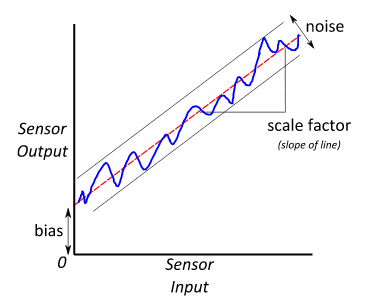
\includegraphics[width=.3\textwidth]{./figs/common_imu_errors.png}
    \caption{一般的IMU误差模型\citep{imu2014}}
    \label{fig:common_imu_errors}
\end{figure}

可以看到,IMU误差的成分是比较复杂的,不同类型误差对于运动估计的影响也是不同的。前面我们提到,在位姿估计的过程中,我们会对角速度$\bm\omega$进行数值积分,得到系统的朝向$\mathrm{R}$,而对加速度$\mathbf{a}$进行一次和二次积分,分别得到速度$\mathbf{v}$和平移$\mathbf{p}$。加速度经过了两次数值积分,其误差也会通过两次积分进入平移量$\mathbf{p}$中,故相比角速度的误差,我们的跟踪算法对于加速度的误差更为敏感。实际经验也告诉我们,由IMU积分得到的朝向信息是较为准确的,而位置信息的误差则是较大的。

不过,一般IMU在出厂时都会经过厂商的校准,故我们可以不必使用上面那样复杂的误差模型。以常用的六轴IMU为例,目前VIO算法中最为常用的做法是将其误差模型简化为偏移和测量噪声两个部分,并假设加速度计和陀螺仪相互统计独立,且各自的三轴之间都统计独立。我们用下标$m$标记每次观测的值,不带下标的表示真实值,在不考虑地球自转的情况下,角速度和加速度的观测量分别为\citep{mourikis2007multi}:

\begin{equation}
\begin{aligned}
    \tilde{\bm\omega} &= \bm\omega + \mathbf{b}^g + \bm\eta^g,  \\
    \tilde{\mathbf a} &= \prescript{G}{}{\mathrm{R}^\top}
                         (\prescript{G}{}{\mathbf a} - \prescript{G}{}{\mathbf g}) +
                         \mathbf{b}^g + \bm\eta^g
\end{aligned}
\end{equation}

使用左上标$^G$来表示全局坐标系,不带左上标的表示当前的局部坐标系。可以看到,IMU的的读数可以看成是真实值、偏移和加性高斯白噪声(addative Gaussian white noise)之和。加速度计又有点特殊,它的读数里面还包含重力$\prescript{G}{}{\mathbf g}$的影响。

另外就是所谓的偏移和白噪声了:
\begin{itemize}
    \item 偏移$\mathbf{b}$随时间的增长符合零均值的高斯随机游走。这个噪声从IMU开机以来就一直存在,不断积累,与是否从IMU读取数据无关。可以用一个初始偏移量$\mathbf{b}_0$和随机游走噪声$\mathbf{n}_w$来描述它:$\mathbf{b} = \mathbf{b}_0 + \mathbf{n}_b$;
    \item 测量噪声$\bm\eta$为零均值的加性高斯白噪声,表示从IMU读取数据时产生的小抖动,而且这个噪声只在观测它的时候产生。
\end{itemize}

其中:

\begin{equation}
\begin{aligned}
    \mathbf{n}_{bg} & \thicksim \mathcal{N}(\mathbf{0}, \mathrm\Sigma_{bg}), &
    \bm\eta_{wg}    & \thicksim \mathcal{N}(\mathbf{0}, \mathrm\Sigma_{wg}), \\
    \mathbf{n}_{ba} & \thicksim \mathcal{N}(\mathbf{0}, \mathrm\Sigma_{ba}), &
    \bm\eta_{wa}    & \thicksim \mathcal{N}(\mathbf{0}, \mathrm\Sigma_{wa}),
\end{aligned}
\end{equation}

故它们的协方差矩阵为:

\begin{equation}
    \mathrm{Q}_{\textrm{IMU}} = \mathbf{diag}(
        \mathrm\Sigma_{bg},
        \mathrm\Sigma_{wg},
        \mathrm\Sigma_{ba},
        \mathrm\Sigma_{wa}
    )
\end{equation}

\subsubsection*{离散时间噪声和连续时间噪声}

上面说的噪声模型都是在连续时间系统下面考虑的,连续时间系统的高斯协方差(或标准差)也就称为传感器的噪声强度。实际上我们不可能每时每刻都在观测IMU,这是一个离散时间系统。离散时间噪声和连续时间噪声的关系,可以参考\citep{smith1978exact}。这里我们只是简单地给出离散时间系统下噪声的协方差。以陀螺仪为例,一般我们会假设我们会假设三轴的噪声独立同分布,假设采样时间间隔为$\Delta t$,那么陀螺仪的两种噪声协方差就是:

\begin{equation}
\begin{aligned}
    \mathrm\Sigma_{bgd} &= \mathrm\Sigma_{bg} \Delta t,  \\
    \mathrm\Sigma_{wgd} &= \mathrm\Sigma_{wg} / \Delta t.
\end{aligned}
\end{equation}

加速度计的形式是一样的。

\subsubsection*{IMU状态传递}

所谓的IMU状态传递(IMU propagation)指的就是根据通过将当前时刻IMU的读数在时间上进行积分,来得到下一时刻的IMU状态。这个IMU状态包括IMU的位姿、运动以及噪声等,通过积分操作,IMU读数的信息就被“传递”到了下一时刻。

我们先来考虑理想情况,也就是IMU的读数不存在白噪声,偏移量也不存在随机游走的情况,此时IMU的读数符合:

\begin{equation}
\begin{aligned}
    \bm\omega  &= \tilde{\bm\omega} - \mathbf{b}^g, \\
    \mathbf{a} &= \tilde{\mathbf a} - \mathbf{b}^a + \mathbf{g}.
\end{aligned}
\end{equation}

记全局坐标系下IMU的状态为(为保持简洁,省略了转置符号${}^\top$):

\begin{equation}
  \mathbf{X}_{\textrm{IMU}} \triangleq
  \left[
      \prescript{G}{}{\mathrm R},
      \prescript{G}{}{\mathbf p},
      \prescript{G}{}{\mathbf v},
      \mathbf{b}^g, \mathbf{b}^a
  \right].
\end{equation}

具体来说,积分过程包括积分这个IMU状态向量的五个分量。那么,要对IMU状态进行积分,我们首先要写出IMU状态关于时间的导数:

\begin{equation}
\begin{aligned}
    \prescript{G}{}{\dot{\mathrm R}}
        &= \prescript{G}{}{\mathrm R} \lfloor(\tilde{\bm\omega} - \mathbf{b}^g)\times\rfloor, \\
    \prescript{G}{}{\dot{\mathbf p}}
        &= \prescript{G}{}{\mathbf v}, \\
    \prescript{G}{}{\dot{\mathbf v}}
        &= \prescript{G}{}{\mathrm R} (\tilde{\mathbf a} - \mathbf{b}^a + \mathbf{g}), \\
    \dot{\mathbf b}^g &= \mathbf{0}, \\
    \dot{\mathbf b}^a &= \mathbf{0}
\end{aligned}
\end{equation}

显然,由于偏移$\mathbf{b}^g$和$\mathbf{b}^a$随时间的增长符合零均值的高斯随机游走,故它们关于时间的导数为零。积分的步骤如下:

\begin{enumerate}
    \item 将角速度在时间上积分,得到当前IMU的朝向;
    \item 将加速度在时间上积分,得到当前IMU的速度;
    \item 将速度再在时间上积分,得到当前IMU的位置;
    \item 角速度偏移和加速度偏移由于增长符合零均值随机游走,所以直接取旧的状态中的值。
\end{enumerate}

我们可以使用任意一种数值积分算法来实现,比如欧拉法(Euler method)、龙格库塔法(Runge-Kutta methods)\citep{wiki2017runge}等。此外,不仅要对状态向量进行数值积分,同时我们还要更新协方差矩阵。

\subsection{优化方法}

近些年来,IMU被广泛地与视觉SLAM系统结合。不管是使用滤波方法还是非线性优化方法实现的VISLAM系统,对IMU的建模都大同小异,基本集中在两类:一类是类似于MSCKF\citep{mourikis2007multi}、OKVIS\citep{leutenegger2015keyframe}那样一般的IMU积分,另一类则是使用IMU预积分的方法,如\citep{forster2017manifold}、VINS\citep{li2017monocular}。

\subsubsection*{基于MSCKF的VISLAM}

MSCKF全称是多状态约束卡尔曼滤波(Multi-State Constraints Kalman Filter),是较早的关于VISLAM的工作。MSCKF使用了一般的IMU积分技术,即通过对IMU读数进行积分,得到作为状态的先验分布,而将图像特征信息作为观测,通过扩展卡尔曼滤波方法求解状态的后验分布。

MSCKF的状态变量实际也是一个状态窗口,它包括最新的IMU状态和保留在窗口内的部分历史相机状态。$k$时刻的状态变量定义如下:

\begin{equation}
    \mathbf{X}_k \triangleq
    \left[
        \mathbf{X}_{\textrm{IMU}_k},
        \prescript{G}{}{\mathrm R}_{C_1},
        \prescript{G}{}{\mathbf p}_{C_1},
        \cdots,
        \prescript{G}{}{\mathrm R}_{C_N},
        \prescript{G}{}{\mathbf p}_{C_N}
    \right]
\end{equation}

MSCKF的算法的框架如下:

\begin{enumerate}
    \item 状态传播:对于IMU读数,使用龙格库塔法对其进行积分,同时根据噪声参数更新状态的协方差矩阵;
    \item 图像注册:每当得到新的图像时,根据当前的最新状态以及IMU-相机外参对状态进行增广,得到状态的先验。并对图像进行处理,提取视觉特征,更新特征跟踪信息等;
    \item 状态更新:选择合适的时机,计算卡尔曼增益,对状态进行更新,得到后验状态信息。
\end{enumerate}

MSCKF算法是无结构信息的,也就是只估计相机/IMU的状态,而不估计三维点的状态。每当要进行状态更新时,选取一部分特征,通过边缘化的操作将它们的信息融合到相机/IMU状态中,然后再对状态进行更新。MSCKF依据两条策略来选取特征,或者说,以下两条规则会触发状态更新:

\begin{itemize}
    \item 这种情况触发地最频繁:当一个视觉特征在被连续跟踪数帧后丢失(移出相机视野)时会触发一次状态更新。这种情况下,由于在最新的相机中特征已经丢失,因此后续它不会再更新,可以通过边缘化操作将它消去。
    \item 第二种情况,每次得到图像时,MSCKF都会增广当前的状态变量,当状态变量中的相机数量达到上限$N_{max}$时,则需要删除一些相机状态。当然,在去除之前,需要先把这些相机参数包含的信息通过状态更新保留下来(边缘化操作)。MSCKF选择从状态中第二老的相机开始,平均选取$N_{max}/3$个相机,这样做是为了尽可能保留长的基线,使得更多的几何信息能被保留下来。选取了相机之后,使用被选中的相机观测到的特征跟踪来更新状态。此后,这几个相机的状态就可以被删除了。
\end{itemize}

\subsubsection*{基于IMU预积分技术的VISLAM}

接下来重点介绍IMU预积分技术\citep{forster2017manifold}。

与普通基于IMU积分的VISLAM系统不同,\citeauthor{forster2017manifold}使用了更精确的相对运动模型。将IMU观测模型包含三个部分:相对旋转、相对速度、相对平移,可以认为它们是仅关于偏移量的函数。使用以下算法进行IMU预积分,假设需要对$t_i$和$t_j$之间IMU读数进行积分(假设相邻两帧IMU之间时间间隔相同,即$\Delta t_{i,i+1} = \Delta t_{i+1,i+2} = \cdots = \Delta t_{j-1,j} = \Delta t$):

\begin{equation}
\begin{aligned}
\mathrm{R}_j &= \mathrm{R}_i \prod_{k=i}^{j-1}
                \bm{Exp}\left(
                    (\tilde{\bm\omega}_k - \mathbf{b}_k^g - \bm{\eta}_k^g) \Delta t
                \right) \\
\mathbf{v}_j &= \mathbf{v}_i + \mathbf{g} \Delta t_{ij} + \sum_{k=i}^{j-1}
                \mathrm{R}_k (\tilde{\mathbf a}_k - \mathbf{b}_k^a - \bm\eta_k^a) \Delta t \\
\mathbf{p}_j &= \mathbf{p}_i + \sum_{k=i}^{j-1}
                \left[
                    \mathbf{v}_k \Delta t +
                    \frac{1}{2}\mathbf{g}\Delta t^2 +
                    \frac{1}{2}\mathrm{R}_k
                    (\tilde{\mathbf a}_k - \mathbf{b}_k^a - \bm\eta_k^a) \Delta t^2
                \right]
    \end{aligned}
\end{equation}

传统的VISLAM中,通常将连续关键帧之间的一系列IMU读数进行积分,得到相对的状态变化“$\Delta\mathbf X$”,然后加上前一个关键帧的状态$\mathbf{X}_i$,得到下一个关键帧的状态$\mathbf{X}_j$,同时计算出累积的协方差,作为下一个关键帧的先验估计,参与到视觉的优化中去。这样做的缺陷就是,积分项$\Delta\mathbf X$实际上会随着偏移量的更新而改变,除非在每一轮优化迭代时重新积分计算新的$\Delta\mathbf X$,否则IMU积分项的误差会一直存在。

按照如下方式定义状态$\mathbf{X}_i$和$\mathbf{X}_j$之间的相对状态变化$\Delta\mathbf X$:

\begin{equation}
\begin{aligned}
    \Delta\mathrm{R}_{ij}
  &\triangleq \mathrm{R}_i^\top \mathrm{R}_j
  = \prod_{k=i}^{j-1}
  \bm{Exp}\left(
      (\tilde{\bm \omega}_k - \mathbf{b}_k^g - \bm{\eta}_k^g) \Delta t
  \right) \\
  %
  \Delta\mathbf{v}_{ij}
  &\triangleq \mathrm{R}_i^\top (\mathbf{v}_j - \mathbf{v}_i - \mathbf{g} \Delta t_{ij})
  = \sum_{k=i}^{j-1}
  \Delta\mathrm{R}_{ik}
  (\tilde{\mathbf a}_k - \mathbf{b}_k^a - \bm\eta_k^a) \Delta t \\
  %
  \Delta\mathbf{p}_{ij}
  &\triangleq \mathrm{R}_i^\top
  \left(
      \mathbf{p}_j - \mathbf{p}_i -
      \mathbf{v}_i \Delta t_{ij} -
      \frac{1}{2} \mathbf{g} \Delta t_{ij}^2
  \right) \\
  &=           \sum_{k=i}^{j-1}
  \left[
      \Delta\mathbf{v}_{ik} \Delta t +
      \frac{1}{2} \Delta\mathrm{R}_{ik}
      (\tilde{\mathbf a}_k - \mathbf{b}_k^a - \bm\eta_k^a) \Delta t^2
  \right]
\end{aligned}\label{eq:raw_int}
\end{equation}

每一轮优化迭代过后,使用一阶的线性方法对$\Delta\mathrm{R}_{ij}, \Delta\mathbf{p}_{ij}, \Delta\mathbf{v}_{ij}$这三个量进行更新,这样就使得在状态变量随着优化在更新的时候,状态的观测也在不断地向着更准确的方向更新,使得整个观测模型更加精准,这也是这篇文章的最大贡献。

\subsubsection*{预积分项的误差模型}

传统的IMU积分其实也可以通过不断地重新积分来不断地使观测模型变精准,但是每次重新积分的计算代价太大了,一般不会这么做。而预积分的基本操作就是首先假设两帧之间的偏移量为定值,即$\mathbf{b}_i = \mathbf{b}_{i+1} = \cdots = \mathbf{b}_{j-1}$,然后将式\eqref{eq:raw_int}的普通IMU积分项认为是与预积分项-白噪声带来的扰动量之和:

\begin{equation}
\begin{aligned}
    \Delta\mathrm{R}_{ij} &\triangleq
        \Delta\tilde{\mathrm R}_{ij}(\mathbf{b}^g_i) \bm{Exp}(-\delta\bm\phi_{ij}) \\
    \Delta\mathbf{v}_{ij} &\triangleq
        \Delta\tilde{\mathbf v}_{ij}(\mathbf{b}^g_i, \mathbf{b}^a_i) - \delta\mathbf{v}_{ij} \\
    \Delta\mathbf{p}_{ij} &\triangleq
        \Delta\tilde{\mathbf p}_{ij}(\mathbf{b}^g_i, \mathbf{b}^a_i) - \delta\mathbf{p}_{ij}
\end{aligned}
\end{equation}

最终可以得到IMU预积分项$[\Delta\tilde{\mathrm R}_{ij},\Delta\tilde{\mathbf v}_{ij},\Delta\tilde{\mathbf p}_{ij}]$和预积分的误差项$\bm\eta_{ij} \triangleq \left[\delta\bm\phi_{ij},\delta\mathbf{v}_{ij},\delta\mathbf{p}_{ij}\right]$,并且认为这个$9$维的误差也是符合均值为零的高斯分布的。记它的协方差为$\mathrm{\Sigma}_{ij}$,即$\bm\eta_{ij} \sim \mathcal{N}\left(\mathbf{0},\mathrm{\Sigma}_{ij}\right)$。而这个协方差,显然是在预积分的过程中通过IMU读数的白噪声累积得来的。因此需要在预积分的过程中根据白噪声的协方差$\bm\eta \triangleq \left[\bm\eta^g,\bm\eta^a\right] \sim \mathcal{N}(\mathbf{0},\mathrm\Sigma_{\bm\eta})$同时也完成白噪声的传递。限于篇幅,白噪声的传递的推导,这里不再给出。

\subsubsection*{偏移量的线性修正}

上面说到,预积分技术使用线性的方法将每轮迭代时偏移量增量更新到预积分项中去,作为其修正。因此需要先将偏移量写成一个偏移量初值加迭代小增量的形式:

\begin{equation}
\begin{aligned}
    \hat{\mathbf b}^g_i &= \bar{\mathbf b}^g_i + \delta\mathbf{b}^g_i \\
    \hat{\mathbf b}^a_i &= \bar{\mathbf b}^a_i + \delta\mathbf{b}^a_i
\end{aligned}
\end{equation}

记$\Delta\bar{\mathrm R}_{ij}\triangleq\Delta\tilde{\mathrm R}(\bar{\mathbf b}^g_i), \Delta\bar{\mathbf v}_{ij}\triangleq\Delta\tilde{\mathbf v}_{ij}(\bar{\mathbf b}^g_i,\bar{\mathbf b}^a_i), \Delta\bar{\mathbf p}_{ij}\triangleq\Delta\tilde{\mathbf p}_{ij}(\bar{\mathbf b}^g_i,\bar{\mathbf b}^a_i)$,按如下方式进行线性修正:

\begin{equation}
\begin{aligned}
    \Delta\tilde{\mathrm R}_{ij}(\hat{\mathbf b}_i^g)
  &\triangleq \Delta\tilde{\mathrm R}_{ij}(\bar{\mathbf b}^g_i + \delta\mathbf{b}^g_i)
  \simeq \Delta\bar{\mathrm R}_{ij}
  \bm{Exp}\left(
      \tfrac{\partial\Delta\bar{\mathrm R}_{ij}}{\partial\mathbf{b}^g_i}
      \delta\mathbf{b}^g_i
  \right) \\
  \Delta\tilde{\mathbf v}_{ij}(\hat{\mathbf b}^g_i,\hat{\mathbf b}^a_i)
  &\triangleq \Delta\tilde{\mathbf v}_{ij}(
  \bar{\mathbf b}^g_i + \delta\mathbf{b}^g_i,
  \bar{\mathbf b}^a_i + \delta\mathbf{b}^a_i)
  \simeq \Delta\bar{\mathbf v}_{ij} +
  \tfrac{\partial\Delta\bar{\mathbf v}_{ij}}{\partial\mathbf{b}^g_i}
  \delta\mathbf{b}^g_i +
  \tfrac{\partial\Delta\bar{\mathbf v}_{ij}}{\partial\mathbf{b}^a_i}
  \delta\mathbf{b}^a_i \\
  \Delta\tilde{\mathbf p}_{ij}(\hat{\mathbf b}^g_i,\hat{\mathbf b}^a_i)
  &\triangleq \Delta\bar{\mathbf p}_{ij}(
  \bar{\mathbf b}^g_i + \delta\mathbf{b}^g_i,
  \bar{\mathbf b}^a_i + \delta\mathbf{b}^a_i)
  \simeq \Delta\bar{\mathbf p}_{ij} +
  \tfrac{\partial\Delta\bar{\mathbf p}_{ij}}{\partial\mathbf{b}^g_i}
  \delta\mathbf{b}^g_i +
  \tfrac{\partial\Delta\bar{\mathbf p}_{ij}}{\partial\mathbf{b}^a_i}
  \delta\mathbf{b}^a_i
\end{aligned}\label{eq:bias_upd}
\end{equation}

这样,在每轮优化迭代的时候,需要同时使用式$\eqref{eq:bias_upd}$,将新的偏移量更新到IMU预积分结果里。不过,当必要的时候,比如偏移量的增量非常大,那么线性更新可能精度也是不够的,此时还是可以采用重新积分的方式去更新预积分项,以减少误差累积。

\subsubsection*{非线性优化}

传统的VISLAM或VIO算法,IMU项参与优化的方式一般非常直接——使用IMU积分得到状态先验,再和视觉观测融合,如此反复。例如OKVIS中的非线性优化(下图是OKVIS优化的因子图)。

\begin{figure}[htb!]
    \centering
    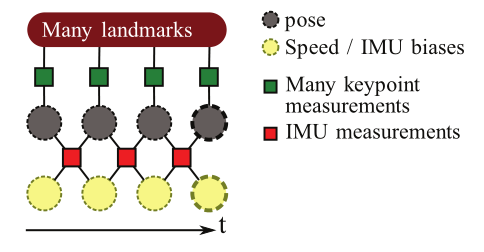
\includegraphics[width=.5\textwidth]{./figs/okvis.png}
    \caption{OKVIS因子图示例图\citep{leutenegger2015keyframe}}
    \label{fig:okvis}
\end{figure}

和大部分的SLAM系统一样,IMU预积分技术的后端优化也是基于非线性最小二乘。它的能量函数同样包括基本的视觉观测项和IMU预积分项(见图\ref{fig:preint}),形式上没有区别,区别仅在IMU部分的能量:

\begin{equation}\label{eq:gtsam_res}
    \bm{\mathcal X}^\star =
        \arg\mathop{\min}_{\bm{\mathcal X}}
        \sum_{i,j}\lVert \mathbf{r}_{\mathcal{I}_{ij}} \rVert^2_{\mathrm\Sigma_{ij}} +
        \sum_{i} \sum_{l} \lVert \mathbf{r}_{\mathcal{C}_{il}} \rVert^2_{\mathrm\Sigma_{C}}
\end{equation}

\begin{figure}[htb!]
    \centering
    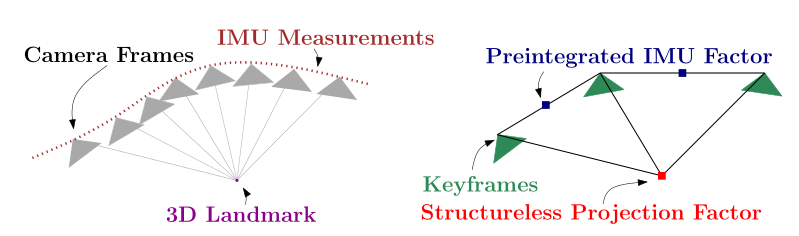
\includegraphics[width=.8\textwidth]{./figs/preint.png}
    \caption{IMU预积分因子图示例\citep{forster2017manifold}}
    \label{fig:preint}
\end{figure}

其中$\mathbf{r}_{\mathcal{C}_{il}}$是关于状态$i$和路标点$l$的视觉残差,这一部分的定义和大部分SLAM系统一致。$\mathbf{r}_{\mathcal{I}_{ij}}$则与MSCKF、OKVIS等系统不同,是关于相邻状态$i$和$j$的IMU预积分残差。在IMU预积分技术中,这一项被认为是仅和状态$i$的偏移量相关的函数:$\Delta\tilde{\mathrm R}_{ij}(\mathbf{b}^g_i)$、$\Delta\tilde{\mathbf v}_{ij}(\mathbf{b}^g_i, \mathbf{b}^a_i)$和$\Delta\tilde{\mathbf p}_{ij}(\mathbf{b}^g_i, \mathbf{b}^a_i)$。前面已经给出了IMU预积分项的误差模型,因此可以很容易地写出IMU预积分项的残差公式:

\begin{equation}
\begin{aligned}
  \mathbf{r}_{\Delta\mathrm{R}}
    &\triangleq
      \bm{Log}\left(
        \left(
          \Delta\bar{\mathrm R}_{ij}
          \bm{Exp}\left(
            \frac{\partial\Delta\bar{\mathrm R}_{ij}}{\partial\mathbf{b}^g_i}
            \delta\mathbf{b}^g_i\right)
        \right) \mathrm{R}^\top_i \mathrm{R}_j
      \right) \\
  \mathbf{r}_{\Delta\mathbf{v}}
    &\triangleq
      \mathrm{R}^\top_i(\mathbf{v}_j - \mathbf{v}_i - \mathbf{g}\Delta t_{ij}) -
      \left[
        \Delta\bar{\mathbf v}_{ij} +
        \tfrac{\partial\Delta\bar{\mathbf v}_{ij}}{\partial\mathbf{b}^g_i}
        \delta\mathbf{b}^g_i +
        \tfrac{\partial\Delta\bar{\mathbf v}_{ij}}{\partial\mathbf{b}^a_i}
        \delta\mathbf{b}^a_i
      \right] \\
  \mathbf{r}_{\Delta\mathbf{p}}
    &\triangleq
      \mathrm{R}^\top_i(
        \mathbf{p}_j - \mathbf{p}_i -
        \mathbf{v}_i \Delta t_{ij} -
        \frac{1}{2}\mathbf{g}\Delta t^2_{ij}) -
      \left[
        \Delta\bar{\mathbf p}_{ij} +
        \tfrac{\partial\Delta\bar{\mathbf p}_{ij}}{\partial\mathbf{b}^g_i}
        \delta\mathbf{b}^g_i +
        \tfrac{\partial\Delta\bar{\mathbf p}_{ij}}{\partial\mathbf{b}^a_i}
        \delta\mathbf{b}^a_i \right]
\end{aligned}
\end{equation}

限于篇幅,关于残差的雅各比矩阵计算,包括预积分项关于偏移量的雅各比矩阵,以及IMU预积分项的协方差矩阵的传递,本书没有给出,有兴趣的读者可以参照原论文进行推导。

\subsection{VISLAM框架}

前面已经讨论了VSLAM的基本框架一般包括初始化、前端跟踪、后端优化(局部和全局优化)、重定位和回路闭合等。而VISLAM一般和VSLAM差异不大,同样也包含这些模块。不过由于多了IMU这个传感器,各个模块的具体行为会有所差异。一个一般的VISLAM框架可以用下图来表示:

正如上图所展示的,它在逻辑上被划分为四个模块:初始化模块、前端视觉惯导跟踪模块、后端非线性优化模块以及一个回环检测模块。

\subsubsection*{初始化模块}

初始化模块的目标是获得初始的状态变量值。与VSLAM相比,VISLAM的状态估计部分由于状态量变多,需要包括初始的旋转(由于重力加速度的值可以认为是不变的,因此初始化计算重力方向即可认为是计算相对于重力的旋转)、速度、尺度、IMU的偏移量。有的系统并没有着重介绍初始化部分,如MSCKF\citep{mourikis2007multi}更依赖后续的滤波算法来使状态收敛,而VINS\citep{li2017monocular}则较为完整的初始化思路,大致策略为使用纯视觉SfM和纯惯导积分对齐的方式计算出初始陀螺仪的偏移量,然后将加速度计的偏移量置为零,并使用一个简化的线性VIO问题来计算初始状态的速度、重力、与SfM结果的相对尺度量。具体的方法可以参考其文章。

\subsubsection*{前端跟踪模块}

通常IMU的频率要远高于相机获取图像的帧率,因此两种传感器之间的时间戳对齐也是VISLAM前端跟踪一个较为棘手的问题。一般可以采用线性插值的方法,以图像的时间戳为准,对IMU的读数进行插值。插值法可以得到同步后的两个图像帧之间的一组IMU读数组成的窗口,这样每当接收到图像的时候,可以先对图像进行关键点提取,维护图像之间的匹配关系。IMU方面,使用前面提到过的积分或预积分技术进行处理。

通常需要在前端跟踪模块里先计算好最新状态的初始值,以供后端优化使用。这一部分可以认为是后端优化的“初始化”。VSLAM中可能会使用五点法、八点法等一系列基于多视图几何的方法来计算本质矩阵或是单应性矩阵,然后通过矩阵分解来得到旋转和平移的初值。而在VISLAM中,由于IMU的存在,纯惯导或是视觉惯导结合的方式是更为主流的方法。可以采用直接IMU积分的方式获取新一帧的初始值,亦或更近一步,在前端求解一个小规模的VIO集束优化问题(如两到三个状态),并将求解的结果作为状态的初值加到后端优化中去。

\subsubsection*{后端优化模块}

后端优化模块可以采用上一小节提到过的带先验信息的局部窗口优化的方法。可以在后端维护一个较长的状态窗口,每当有新的状态加入到窗口中时触发一次非线性优化求解。在基于关键帧的VSLAM中,通常只需要根据图像本身来考虑关键帧的筛选,比如特征是否丰富、特征分布是否合理,与上一帧是否能形成足够的视差和共视等。在窗口滑动的时候也有不同的做法:顺序滑动,或用最新的状态替换窗口中最新的状态。离开窗口的状态则以边缘化的方式滑出窗口,其结果会作为先验信息加入到后续优化中。

而在VISLAM中,除了要保证关键帧本身的图像质量和关键帧之间的视差,还要考虑IMU的影响。由于IMU积分模型的模型采用了大量的近似,其模型误差是比较大的。同时考虑到各方面的噪声以及多重积分带来的误差放大效应,移动端常用的消费级IMU通常只在较短的时间窗口内能保证积分的精度。故在选择关键帧时,关键帧之间的IMU窗口不宜过长。

VISLAM的视觉跟踪要求足够的视差,而惯导部分要求较短的时间窗口,这就形成了一些挑战,比如AR应用中时常会遇到低速运动情况,这时候连续帧图像差异比较小,足够的视差通常就意味着较长的IMU窗口。这时候就需要开发者根据实际情况合理设置关键帧筛选策略。

\subsubsection*{回环检测模块}

回环检测模块可以在检测到回路闭合时调用全局集束优化,消除长时间跟踪的积累误差。但是出于性能上的考虑,全局集束优化的不适合频繁地调用。一种策略是在检测到回路闭合之后,将匹配到的历史关键帧加入到当前的滑动窗口中,并设置为固定的变量。这样,窗口内的集束优化就成了以历史关键帧为条件的极大似然估计。另一方面,又可以在额外维护一个全局的集束优化模块,定期运行以消除历史关键帧的误差。这样可以节省大量计算,同时不会引入很大的误差累积。

这个额外的集束优化同样可以采用上一章介绍的一些方法来加速:无结构的位姿图优化、利用全局优化的局部性开发高效的增量优化算法等。
